We have decided to use trace files to obtain information from applications because we wanted to keep AGIOS generic and easy to use. Most methods to obtain such information include changes in I/O libraries, compilers or applications, which would compromise the portability of our tool. The trace file is generated by the scheduler itself and stored on its local storage device, without modifications to the application or to the file system.

\begin{figure}[!b]
\centering
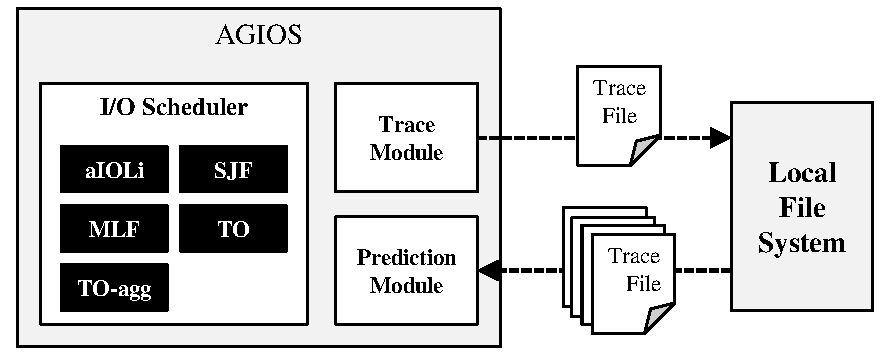
\includegraphics[width=\columnwidth]{images/agios_architecture.pdf}
\caption{AGIOS' modules and trace generation.}
\label{fig:agios_architecture}
\end{figure}

Figure~\ref{fig:agios_architecture} presents AGIOS' modules. 
Trace generation is activated by a configuration parameter, and can be used with any of the provided scheduling algorithms. The \emph{Prediction Module} is responsible for obtaining information from traces and providing them to scheduling algorithms.

The Prediction Module is initialized by the scheduler in the beginning of its execution if trace files are present. A prediction thread then reads the traces and generates a set of queues identical to the ones used during execution, except that these contain ``predicted'' future requests. This initialization can also be triggered during execution, providing the ability to generate a trace file during some initial period of the execution and then start the Prediction Module if we expect the traced access pattern to happen again in the future. This would be done through the \emph{agios\_reset\_stats} call, discussed in Chapter~\ref{chapter:starting}.

\section{Trace generation}

In the trace file, a ``new request'' entry stores the file identifier, offset, size, and timestamp of the request - the number of nanoseconds elapsed since the current trace's first request arrival, or $0$ in the case of the first request. 

Since writing information about requests to a local file could affect the scheduler's results, the Trace Module keeps a buffer. A large trace buffer minimizes the number of I/O operations to the trace file. On the other hand, a buffer that is too large could affect the whole I/O service's performance by increasing its memory footprint.

Different traces generated by executing the same application may present some variation between the arrival times of the same request. In order to obtain more realistic arrival time estimations, several trace files can be combined. Therefore, while reading predicted requests from trace files, the Prediction Module checks if they already exist in its queues. This comparison is done by file identifier, offset, size, and arrival times relative to the first request to the file. Requests are the same only if their arrival times difference is within a tolerance, provided from configuration parameters.

\section{Predicted aggregations}

From a set of predicted future requests, the Prediction Module can predict aggregations that will be possible during execution and provide this information to scheduling algorithms. These predictions require an $\alpha$ factor which represents the ability to overlap waiting times with processing requests from other queues. It is estimated at initialization time, and can be updated during execution time based on the real ability observed at the scheduler.

When an actual request arrives, the scheduler looks for predicted requests to the same file with the same offset, size and with a relative timestamp (relative to the first request to this file) within acceptable bounds. These ``acceptable bounds'' are defined by an acceptable error parameter, the same used while reading traces to decide if predicted requests are the same. If the scheduler finds such a request, the two versions (predicted and actual) are linked and the predictions concerning this request will be considered during scheduling. 

When a virtual request is selected to be served, the scheduler asks the
Prediction Module if it should be done now, or if it should wait
for some period. In order to make this decision, the Prediction Module
analyzes the aggregation predicted for the requests' traced versions. If the aggregation is not as big as the predicted one, the scheduler must wait. In order to avoid starvation, the wait will happen only once for each virtual request. 

This process, available only for I/O scheduling algorithms that have waiting times (aIOLi and MLF), is illustrated in Fig.~\ref{fig:scheduling_traces}. 
In the instant $t_1$, the scheduler needs to decide if it dispatches
    the three highlighted incoming requests for execution or if it waits for
    longer. With information from the trace, the scheduler knows that a bigger aggregation is possible for these requests.

\begin{figure}[!h]
  \centering
  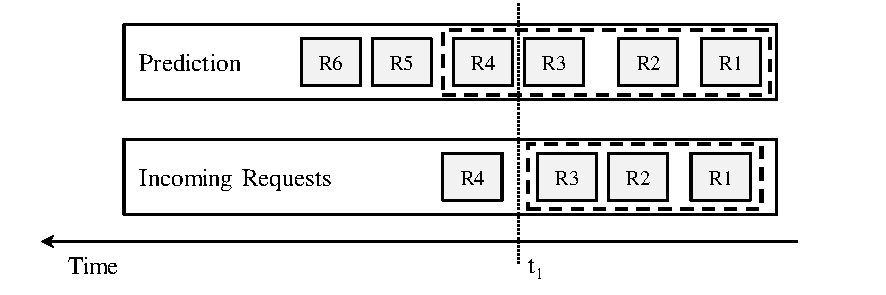
\includegraphics[width=\columnwidth]{images/app_sched.pdf}
  \caption{Scheduling with predicted future requests.}
  \label{fig:scheduling_traces}
\end{figure}

After processing actual requests, predicted versions will not be discarded. Therefore, repeating access patterns (or repeated executions of the same application) can benefit several times from the same predictions. Traces can be reused for applications' executions with different parameters as long as they do not change what file portions are accessed from each server.

\section{Access pattern detection}

Another functionality of the Prediction Module is access pattern detection. Through a decision tree (generated with machine learning techniques), it classifies applications' accesses in contiguous or non-contiguous and small or large. This decision is made from two metrics calculated to each file with predicted accesses. The general access pattern is considered to be the access pattern for the majority of the files.

The process of reading multiple trace files and combining them to generate predictions can be very time consuming. It is possible to enable the generation of simplified trace files by the Prediction Module. These files are generated after reading regular trace files and each one of them has the calculated metrics to a file with predicted requests. In future executions of AGIOS, it is possible to provide only these files (instead of the regular trace files). They will provide enough information to access pattern detection and scheduling algorithm selection, but not for predicting request aggregations.

\section{Scheduling algorithm selection}

The Prediction Module is also capable of selecting automatically the best fit in scheduling algorithm depending on the situation. This is also done through a decision tree, using the detected general access pattern and information about the storage device. For now, this selection is only available at initialization time, using information from traces.

Information about the storage device is obtained through .h files generated by SeRRa. This will be further discussed in the next chapter.

Both the access pattern detection and scheduling algorithm selection were designed for AGIOS' use by a parallel file system's data servers. For other situations, results should make no sense, so please avoid using these functionalities.

